\chapter{Technical Foundation} \label{tech}
\section{Finite Element Method}\label{femsec}
Finite element methods (or finite element analysis) is used when the behaviour of an element cannot be accurately depicted by a simple mathematical equation. 
	\subsection{Origin}
	The finite element method (FEM) used today is the sum of decades of research. 
	In an article by \citeauthor{Gupta:1996} they discuss the five main contributors to the finite element method. 
	According to \citet{Gupta:1996} the idea behind the finite element method was initially explored in the \citeyear{Courant:1943} article by \citeauthor{Courant:1943}. 
	Courant acknowledges the complex nature of mathematical problems in his first paragraph by stating: "Mathematics is an indivisible organism uniting theoretical contemplation and active application."
	He goes on to discuss the variational method created by (Ryes?)
	
	
	
	\subsection{}
	A larger element is broken into smaller elements. 
	Assumptions made on the smaller scale have a lesser effect on the final answer than the same assumptions made on a large scale would have had.


	\subsection{Heat diffusion}	 
	 In its simplest form, the one-dimensional heat diffusion equation is a partial differential equation \ref{heat_eq} dependant on the temperature and thickness of the element. 
	The heat diffusion equation is based on Fourier's Law...(TODO)
	
	
	\begin{equation}
	\label{heat_eq}
		q = -k \frac{dT}{dx}
	\end{equation}
	\subsection{Heat conduction}
	TODO: - Explain Galerkin Weak form, Newmann boundaries and Dirichlet Boundaries

\section{Bayes' theorem of inverse problems}
%	Statistical and Computational Inverse problems by Kaipio and Somersalo Chapter 3
% 	The Bayesian approach to Inverse Problems Dashti and Stuart
	The method of statistical inversion is dependant on a fundamental understanding of the Bayes' theorem of inverse problems. 
	The student obtained this understanding through studying Chapter 3 of statistical and Computational Inverse problems by \citet{Kaipo:2005}, further referred to merely as Kaipio. 
	There are four principles of Statistical inversion that is essential to the thorough understanding of these models. 
	Firstly, it is the principle that any variable in the model needs to be modelled as a random variable. 
	This randomness is based on the extent of information that is available. 
	To ensure that the extent of knowledge is accurately portrayed in the model, the extent of knowledge will be coded into the probability distributions assigned to the different variables. 
	Finally, it needs to be understood that the solution of a statistical inversion is a posterior probability distribution.
	A generalized equation of Bayes' theorem can be seen in \ref{bayes_eq} taken from Kaipio. 
	
	\begin{equation}
	\label{bayes_eq}
	\pi_{\text{post}}(x) = \pi(x|y_{\text{observed}}) = \frac{\pi_{\text{pr}}(x) \pi(y_{\text{observed}}|x)}{\pi (y_{\text{observed}})}	
	\end{equation}

\section{Markov Chain Monte Carlo} \label{MCMCdet}
Markov Chain Monte Carlo (MCMC) is a method of integration which will be used to determine the mean of the $\kappa$-values at specific temperatures. 
	Markov Chain Monte Carlo is a method that was created by combining the concept of Monte Carlo sampling  and a Markov Chain. 
	To fully understand MCMC, its underlying methods must be investigated further.
	For a better understanding of this concept, \textit{Introducing Markov chain Monte Carlo} by \citeauthor{Gilks:1996}, Kaipio, and various websites \cite{MLM:2019}, \cite{dummies:2015} were consulted.(RIJK: is sin lomp?)
	\subsection{Markov Chains}	
	The core principle of a Markov chain is that the next value ($x_{n+1}$) in a sequence is dependent on the current value($x_n$). 
	This concept can be visualised as follows: our accepted point ($x_1$) is in the center of a cube. The next possible random point is randomly generate but still within the cube. 	
	After this next number is selected, the cube moves such that the new point($x_2$) is now the centre, and so it continues.
	See Figure \ref{cubeexplfig} for clarification.
	The above example simplifies the concept, but this understanding can now be expanded.
	If every coordinate direction in the aforementioned simple example is seen as a single entry in the $x$ vector, then the example has only three $\kappa$-values.
	Another level of complication can be added if it is taken into account that every point in the cube is no longer equally likely.
	A distribution within the cube can be chosen, for example simply a normal distribution
	The shape of the cube then warps into a stranger shape with points closer to the center being more likely choices and the edges being less likely.
	\begin{figure}	
	\centering
	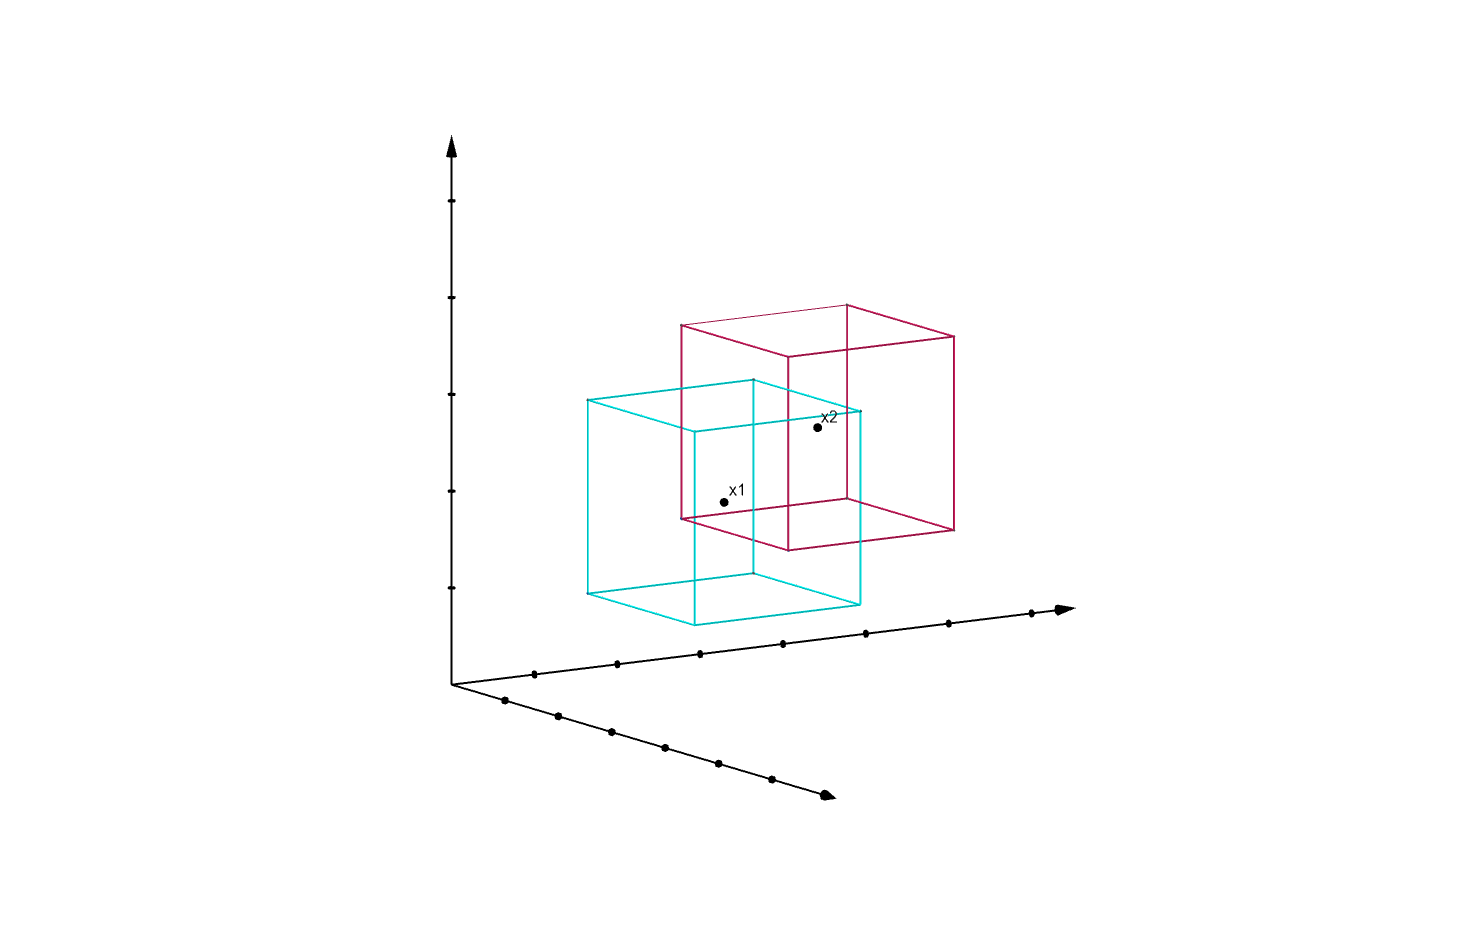
\includegraphics[width=0.55\linewidth]{figures/MC_cubes.png}
	\caption{Three-dimensional example of Markov Chain application (Created on \url{https://www.geogebra.org/3d})}
	\label{cubeexplfig}
	\end{figure}
	
	%%BURN_IN TODO
	The purpose of a Markov Chain is for the chain to converge to a distribution and be independent on the very initial estimation. 
	In principle it should then reach a near stationary distribution.
	Since Markov Chains are not used if we know the answer, a way to determine when values are no longer affected by the initial estimate is needed \cite{Gilks:1996}. 
	The simple proposed solution is the concept of burn-in. 
	The concept of conventional burn-in for usage in Markov Chains are disputed as the Markov Chain itself is created in such a way that values are only directly dependent on the value immediately before them \cite{Meyn:1993}.
	Burn-in in the Markov Chain sense can simply be referred to as the removal of the initial samples of low probability to increase the accuracy of the average taken after all the iterations \cite{John:2016}.
	
	
	
		
	\subsection{Monte Carlo Integration}\label{MCint_sec}
	Monte Carlo integration is used to evaluate a probability distribution that cannot be solved simply. 
	The evaluation is done by drawing a collection of random values from the distribution.
	These values are then used as the sample, and a sample mean is taken.
	The arithmetic sample mean can be used to approximate the population mean in accordance with the law of large numbers \citep{Gilks:1996}.
	All of the random samples generated can not be immediately accepted.
	Here, the acceptance criteria comes into play.
	There are multiple options for how a posterior is deemed acceptable; these are elaborated on in the book  \textit{Monte Carlo Statistical Methods} by \citeauthor{Robert:2004}. 
	The most general acceptance criteria is set out in Equation \ref{acceptcriteq} and comes from Kaipio.
	
		\begin{equation} \label{acceptcriteq}
		\begin{aligned}
		&\text{if  }\quad \frac{\pi (x_2)}{\pi(x_1)} > 1 \quad \text{Accept automatically}\\
		&\text{or  }\quad \frac{\pi (x_2)}{\pi(x_1)} > \text{rand}  \quad \text{Accept}\\
		&\text{else reject and reselect  } x_2
		\end{aligned}
		\end{equation}
	

\subsection{Metropolis-Hastings Algorithm}

The Metropolis-Hastings algorithm is one of the available simulation methods based on the MCMC principles. 
For the purposes of this project the Metropolis-Hastings algorithm was chosen above the Gibbs-sampler TODO


\section{Thermal properties of timber}
